%!TEX TS-program = xelatex
%!TEX encoding = UTF-8 Unicode

\documentclass[12pt]{article}
\usepackage{geometry}                % See geometry.pdf to learn the layout options. There are lots.
\geometry{a4paper,top=2cm}
\usepackage[parfill]{parskip}    % Activate to begin paragraphs with an empty line rather than an indent
\usepackage{graphicx}
\usepackage{amsmath}
\usepackage{amssymb}
\usepackage{physics}
\usepackage{polyglossia}
\setdefaultlanguage{portuguese}

\usepackage{fontspec,xltxtra,xunicode}
\usepackage{unicode-math}
\defaultfontfeatures{Mapping=tex-text}

\title{Mecânica Quântica Avançada\\%
Prova 01\\%
27 de abril -- 08 de maio}
%\author{The Author}
\date{}

\begin{document}
\maketitle
\vspace*{-4em}

\textbf{Exercício 1:} considere uma molécula constituída de três átomos idênticos nos sítios (vértices) de um triângulo equilátero, conforme mostrado na figura.
Vamos considerar que o íon desta molécula é formado adicionando-se um único elétron a ela;
como vimos em aula, deve haver um efeito de delocalização, e o elétron deve se acomodar em um estado distribuído ao redor dos sítios.
Suponha que o elemento de matriz da Hamiltoniana para o elétron em dois sítios adjacentes $i,j$ é $\langle i|H|j \rangle = -a, a>0$, para $i \neq j$; por simetria, os elementos diagonais são todos iguais, $\langle i|H|i\rangle = E_0$.

\begin{center}
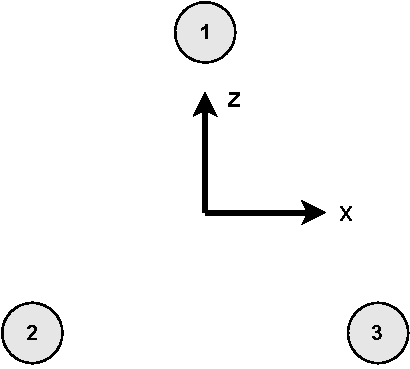
\includegraphics[width=0.24\textwidth]{Figures/EquilateralTriangleMolecule.drawio.pdf}
\end{center}

\textbf{(a)} Escreva a Hamiltoniana na forma matricial e calcule os níveis de energia
$\{E_1^{(0)}, E_2^{(0)}, E_3^{(0)}\}$. 
Deixe tudo em função das variáveis $E_0$ e $a$.

\textbf{(b)} Suponha que um campo elétrico na direção $z$ é aplicado, 
de modo que a energia potencial para o elétron na posição rotulada por ``1'' diminui por uma parcela $b$ ($b > 0$).
Calcule os níveis de energia
$\{E_1, E_2, E_3\}$
e os autoestados de energia.
Deixe tudo em função das variáveis $E_0$, $E_1$, $E_2$ e $a$.

\textbf{(c)} Suponha que, no caso do item (b), o elétron está no estado fundamental.
Quase-instantaneamente, o campo roda de 120\textsuperscript{o} e passa a apontar na direção rotulada como ``2''.
Calcule a probabilidade do elétron permanecer no estado fundamental.
Deixe tudo em função das variáveis $E_0$, $E_1$, $E_2$ e $a$.

\textbf{Exercício 2:} para cada estado $\ket{\psi}$ de dois spins-$\frac{1}{2}$ abaixo, 
escrito em termos dos autovetores de $S_z$, diga se o estado é emaranhado ou não (justificando sua resposta), 
calcule seu operador estado (matriz densidade) explicitamente,
e calcule o operador estado reduzido referente à particula 1 (na notação $\ket{1,2}$).

\textbf{(a)} $\displaystyle\ket{\psi} = \frac{1}{\sqrt{2}}(\ket{+-}-\ket{-+})$.

\textbf{(b)} $\ket{\psi} = \ket{++}$.

\textbf{(c)} $\displaystyle\ket{\psi} = \frac{1}{5\sqrt{2}}
\left(\ket{++} + 3i\ket{+-} - 2i\ket{-+} + 6\ket{--}\right)$.

\clearpage

\textbf{Exercício 3:} Considere um \emph{ensemble} estatístico de sistemas de um spin-$\frac{1}{2}$.

\textbf{(a)} Considere que o ensemble é um estado puro, apontando em uma direção $\hat{n}$ (ver figura), e descrito por um ket $\alpha$. Suponha que os valores esperados $\ev{S_x}$ e $\ev{S_z}$ são conhecidos. 
Construa explicitamente, em termos desses valores esperados, a matriz densidade $2\times2$ que descreve o sistema.

\medskip

\begin{minipage}{0.35\textwidth}
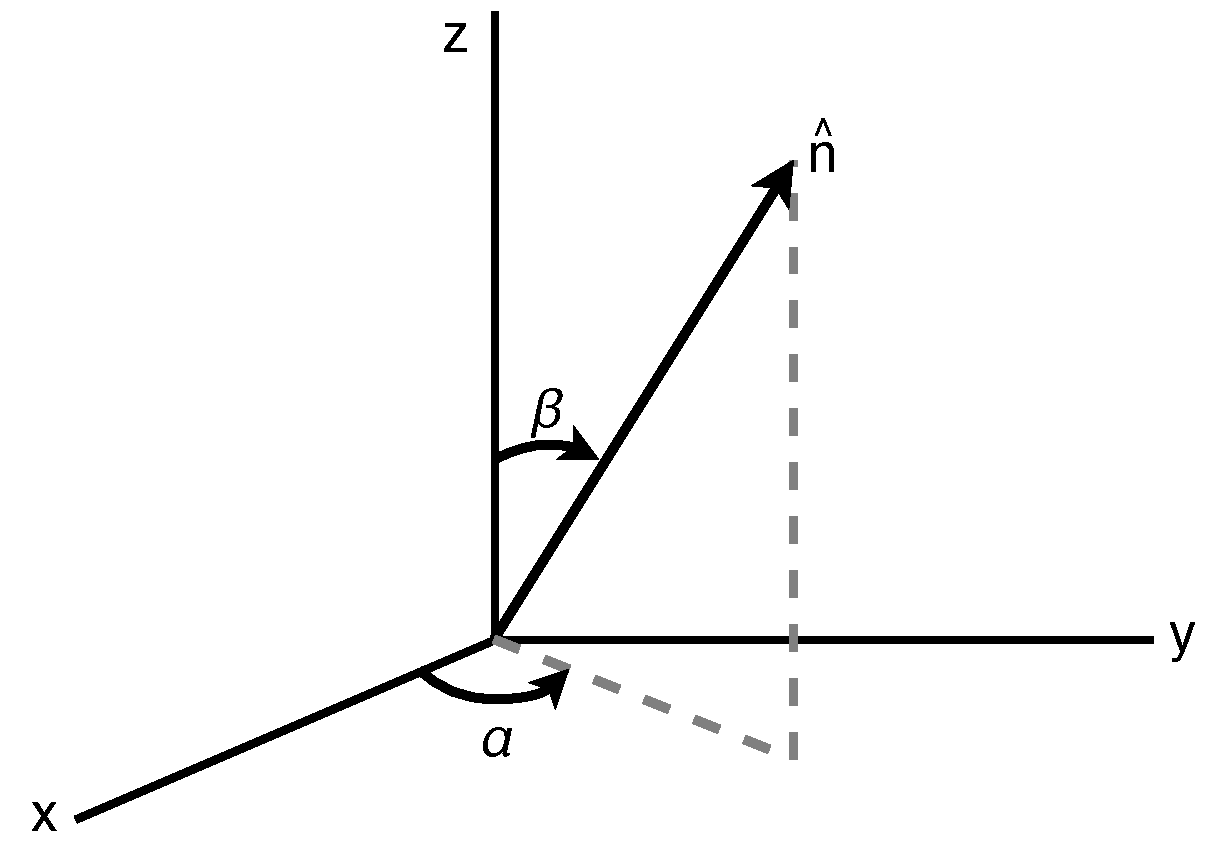
\includegraphics[width=\textwidth]{Figures/nVersor.pdf}
\end{minipage}%
\begin{minipage}{0.65\textwidth}
Estado puro apontando na direção $\hat{n}$:
\[
|\alpha\rangle=\cos \left(\frac{\beta}{2}\right)|+\rangle+e^{i \alpha} \sin \left(\frac{\beta}{2}\right)|-\rangle
\]
\end{minipage}

\medskip

\textbf{(b)} Considere agora que o ensemble é misturado, de uma maneira genérica 
(note que não estamos dizendo que ele é o estado de máxima entropia!). 
Suponha agora que os três valores médios
$\ev{S_x}$, $\ev{S_y}$, $\ev{S_z}$ são todos conhecidos.
Construa explicitamente, em termos desses valores esperados, a matriz densidade $2\times2$ que descreve o sistema.

\vspace*{1em}

\textbf{Exercício 4:} Considere a seguinte matriz densidade de dois spins-$\frac{1}{2}$:
\[
\rho=\frac{1}{8} \mathbb{1}+\frac{1}{2}\left|\Psi_{-}\right\rangle\left\langle\Psi_{-}\right|
\]
onde \(\left|\Psi_{-}\right\rangle\) é o estado singleto (\textit{i.e.} o estado de spin total igual a zero). Suponhamos que
medimos um dos spins ao longo de um eixo \(a\) e o outro ao longo de um eixo \(b\), em que
\(\hat{a} \cdot \hat{b}=\cos \theta\). Qual é a probabilidade (como função de \(\theta\)) de encontramos \(+\hbar / 2\) para ambos
spins nestas medidas?

\textbf{Exercício 5: Interferometria de Ramsey.} Suponha que um sistema de dois níveis tem estados $\ket{+}$ e $\ket{-}$, análogo ao spin-$\frac{1}{2}$

\textbf{(a)} Vamos considerar a chamada interação de \textit{beam splitter (BS).} Suponha que o sistema é sujeito a um Hamiltoniano $H = \epsilon \sigma_y$ por um tempo $\tau$ tal que $\epsilon \tau /\hbar = \pi/4$.
Mostre que se o sistema estava inicialmente em $\ket{+}$ ou $\ket{-}$, então ele é levado (a menos de uma fase global) para os estados:
\[
\ket{+} \to \frac{\ket{+} + \ket{-}}{\sqrt{2}}
\quad,\quad
\ket{-} \to \frac{\ket{+} - \ket{-}}{\sqrt{2}}.
\]

\textbf{(b)} Agora, consideremos a chamada \textit{phase shift gate (PS)}. Suponha agora que o sistema é sujeito a um Hamiltoniano $H = \epsilon \sigma_z$ por um tempo $\tau$ tal que $\epsilon \tau /\hbar = \phi/2$. Mostre que isso leva os vetores (a menos de uma fase global) em
\[
\ket{+} \to \ket{+}\quad,\quad\ket{-} \to \exp(i\phi)\ket{-}.
\]

\textbf{(c)} Considere um sistema inicialmente preparado em $\ket{\psi_0} = \ket{+}$. Suponha agora que esse sistema evolui por um beam splitter, seguido de um phase shift, seguido de outro beam splitter, evoluindo até um estado $\ket{\psi}$. (Note que isto é possível em laboratório, usando exatamente um sistema de spin-$\frac{1}{2}$ e um campo magnético dependente do tempo.)
\[
\ket{\psi_0} \to BS \to PS \to BS \to \ket{\psi}
\]
Calcule o estado final $\ket{\psi}$. 

\textbf{(d)} Mostre que a probabilidade $P_1$ de encontrar o sistema no estado $\ket{-}$ depois da evolução é dada por
\[
P_- = |\bra{-}\ket{\psi}|^2 = \sin^2(\phi/2).
\]
Essa é a ideia principal por trás da interferometria de Ramsey: a probabilidade oscila
dependendo da fase do phase shift.

\end{document}

\vfill
\par\noindent\rule{\textwidth}{0.4pt}


\textbf{Formulário}

Matrizes de Pauli:
\[
\sigma_x = \begin{pmatrix}0&1\\1&0\end{pmatrix},\,
\sigma_y = \begin{pmatrix}0&-i\\i&0\end{pmatrix},\,
\sigma_z = \begin{pmatrix}1&0\\0&-1\end{pmatrix}\quad
\begin{aligned}
\left[\,\sigma_{i}\,, \sigma_{j}\,\right]&=2 i \varepsilon_{i j k} \sigma_{k}\\
\left\{\sigma_{j}, \sigma_{k}\right\}&=2 \delta_{j k}\mathbf{I}
\end{aligned}
\]

Exponencial com matrizes de Pauli: $\exp (i \theta \vec{v} \cdot \vec{\sigma})=\cos (\theta) I+i \sin (\theta) \vec{v} \cdot \vec{\sigma}$

Evolução temporal: $\ket{\psi(t)} = \exp(\frac{-i\hat{H}t}{\hbar}) \ket{\psi(0)}$

Matriz densidade: $\hat{\rho} = \sum_\alpha p_\alpha\op{\varphi_\alpha}{\varphi_\alpha}$; lembre que $\hat{\rho}=\hat{\rho}^{\dagger}$, $\Tr\hat{\rho} = 1$.

Valor médio $\!\ev*{\hat{A}}=\Tr(\hat{\rho}\hat{A})$.

Para sistema de dois níveis:
\[\rho = 
\begin{pmatrix}
a & c\\c^*& 1-a
\end{pmatrix},\,a\text{ real},\,c\text{ complexo}
\]
\end{document}